\ctable[caption={Studying a problem at multiple scales},
		label={fig:scales},
		figure]{c}{\tnote[]{}}{\FL
			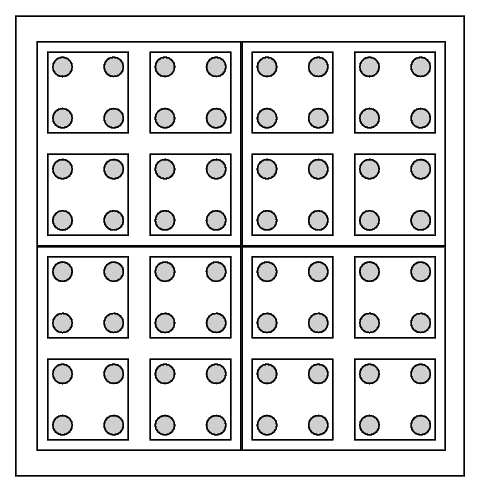
\includegraphics[scale=0.2]{fig/ising.png}
		\LL}
The heart of our method for solving the TSP problem is the renormalization theory. The Renormalization Theory is originating from theoretical physics. In theoretical physics Renormalization is used to study the observe the changes in a physical system. The changes are observed by looking to the problem at different scales. This idea is illustrated in figure \ref{fig:scales}. Here the problem is divided into four parts initially. These parts on their own can again be divided into four parts. This dividing process is repeated until the scale is small enough to study the original problem.

This idea is mapped onto the Traveling Salesman problem. The total square in figure \ref{fig:scales} can be seen as the total area where the cities are located. When estimating the shortest route, we start at a large scale, and we keep zooming in until our estimated optimal tour is known. The procedure is illustrated in figure \ref{fig:renormalization}. The image A is the basic block. This basic block consists of four cells, and can be seen as the four parts in which we divide the problem when we go to a smaller scale. A cell spans a part of the area, and can be enabled or not. The cell is enabled (e.g. needs to be visited) if one or more cities are located in the area spanned by the cell.

The general idea of the algorithm is to solve the Traveling Salesman problem for the larger block. This can be done easily, since a Traveling Salesman problem for at most four cities can be easily solved without much performance penalty, by simply enumerating all possibilities. When this is done, we can look to the TSP at a smaller scale, by dividing the block into four subblocks. Together with some information acquired from the larger block, the Traveling Salesman problem can again be solved for the four subblocks. This process is repeated until there is at most one city in a cell, and the estimated optimal tour is known. In the following subsection we will describes the algorithm in more detail.

\subsection{Preprocessing step}
\ctable[caption={An illustration of how the Renormalization algorithm works},
	label={fig:renormalization},
	figure]{c}{\tnote[]{
	(A) Determine the optimal route in a basic two by two cell. The dashed lines are the edges which can be traversed. The open circles are border points and the closed circles are cell points.\\
	(B) Based on the starting and end border node in a block, lookup the optimal path visiting the cells where at least one city is located.\\
	(C) Divide the block into four subblocks, use the crossings of the route with the borders of a cell (The X) as new starting and end nodes.\\
	(D) These subblocks are treated as a block again, and the process restarts from picture B. This dividing continues until at most one city is in each cell.}}{\FL
	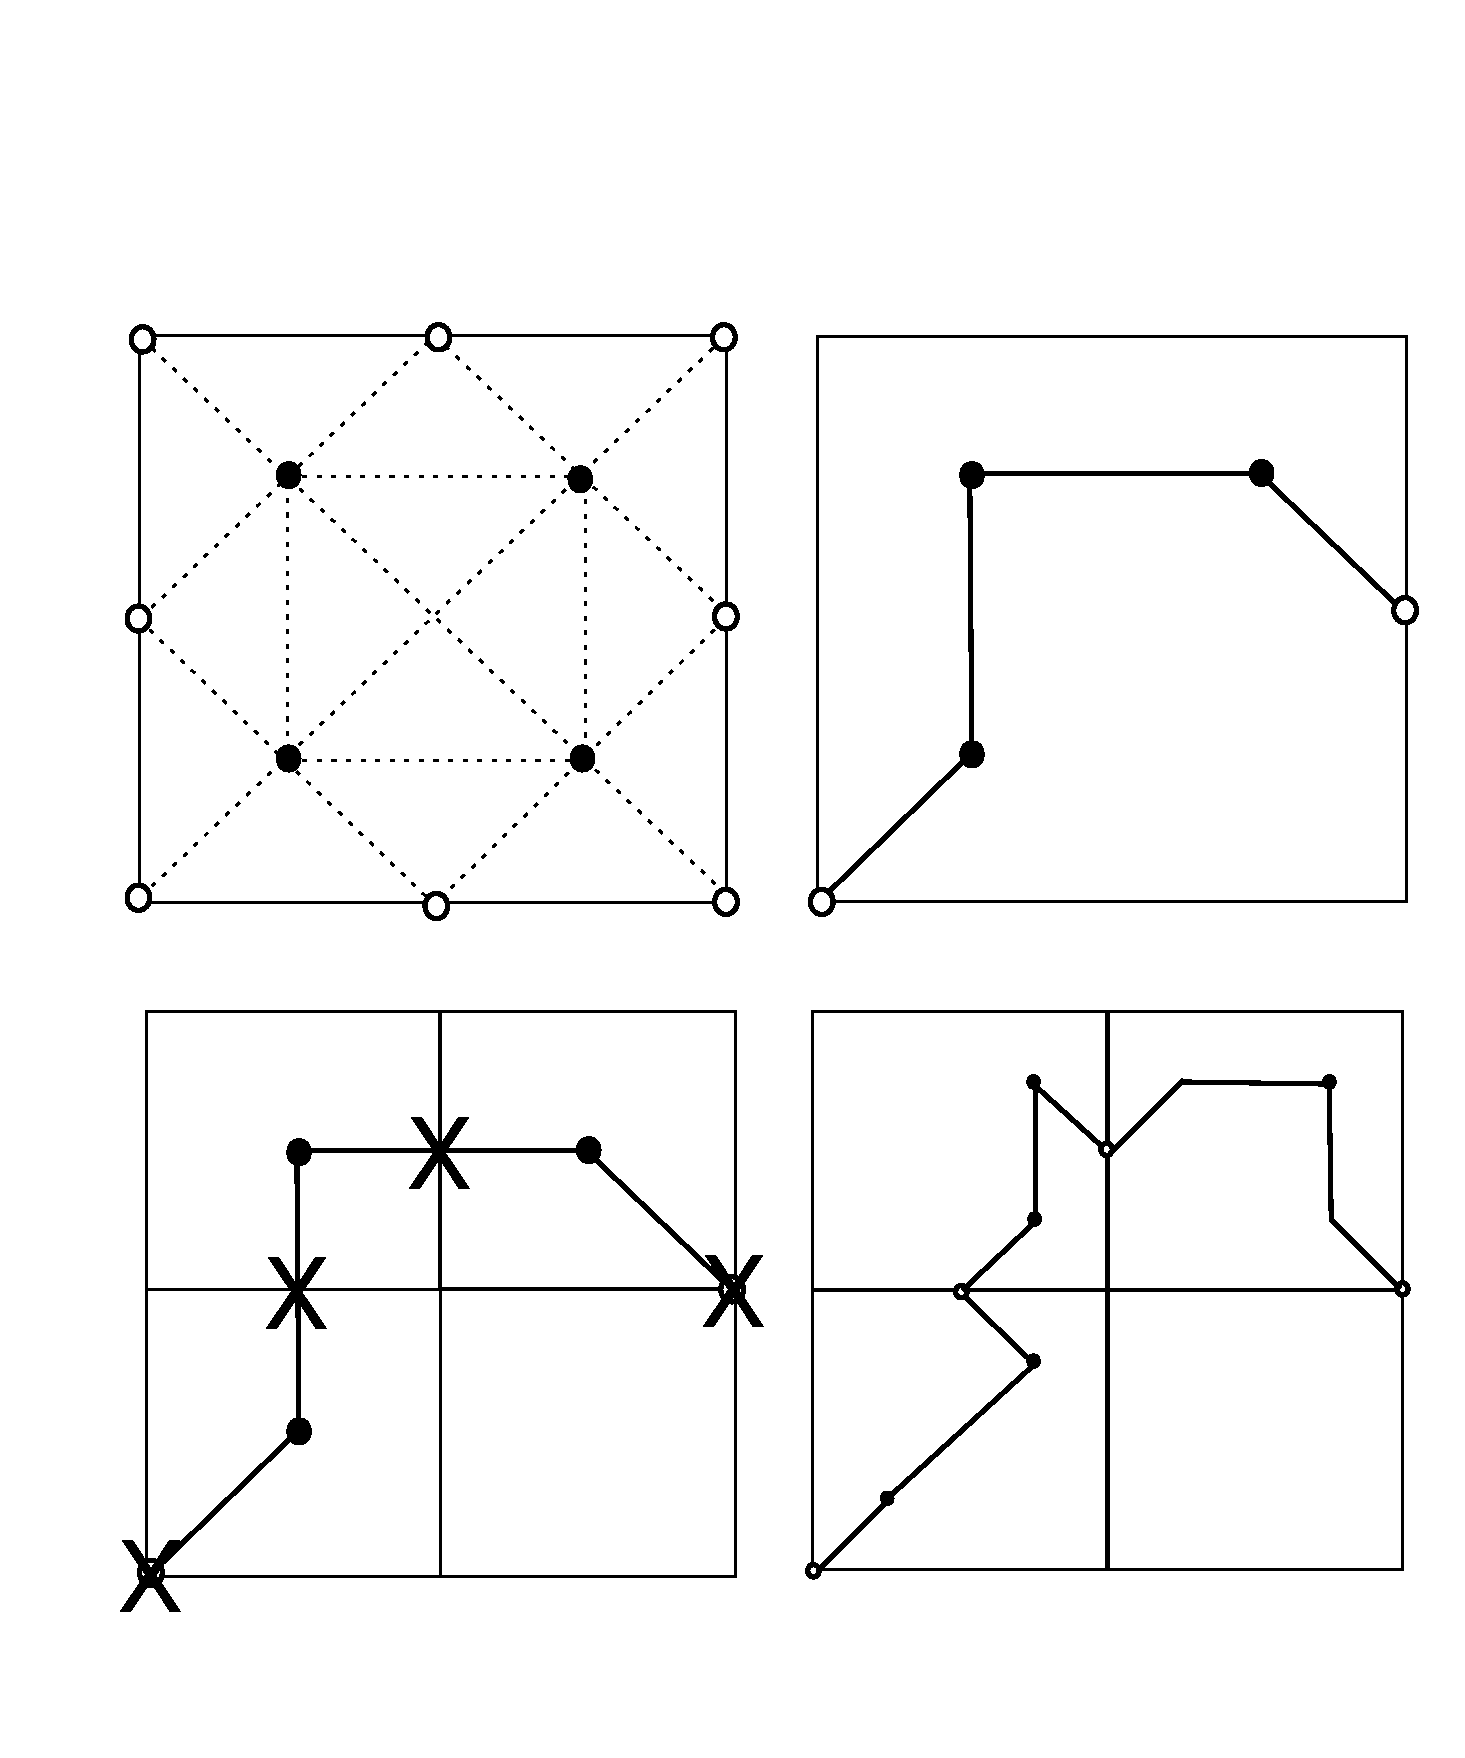
\includegraphics[width=7cm]{fig/renormalization.pdf}
	\LL}

The preprocessing step reduces the amount of calculation needed each time you need to calculate an optimal route in a block. Basically this means that for every possible configuration you calculate the optimal path, and store this in a lookup table. There are two aspects which can be altered, the border point at which the beginning and finish of the route is located and the visited cells within the block.

For retrieving the shortest route through a block, it is considered as a graph. The nodes are the border points and the cell points (Lying in the centrum of a cell). The nodes are connected by multiple edges. There are edges between the border points and the closest cell points. There are also edges from a cell point to the other edges. This set-up can be seen in figure \ref{fig:renormalization}A. For getting the shortest route, a breadth first search is used. Here all possible paths, without cycles, between the starting and end node are calculated. Using these set of paths, the shortest routes visiting subsets of cell points are searched.

\subsection{First iteration}
In the first iteration we start with one block with four cells. In such a block a subset of at least 3 cells needs to be occupied to form a starting tour. The cells where at least one city is located, are connected to form a shortest tour. This tour is an easy connection of the cities, and all the possible routes between them do not need to be investigated.

\subsection{Further iterations}
\ctable[caption={The first four iterations on d198.tsp},
		label={fig:iterations},
		width=7.5cm,
		figure]{cc}{\tnote[]{Some comments}}{\FL
			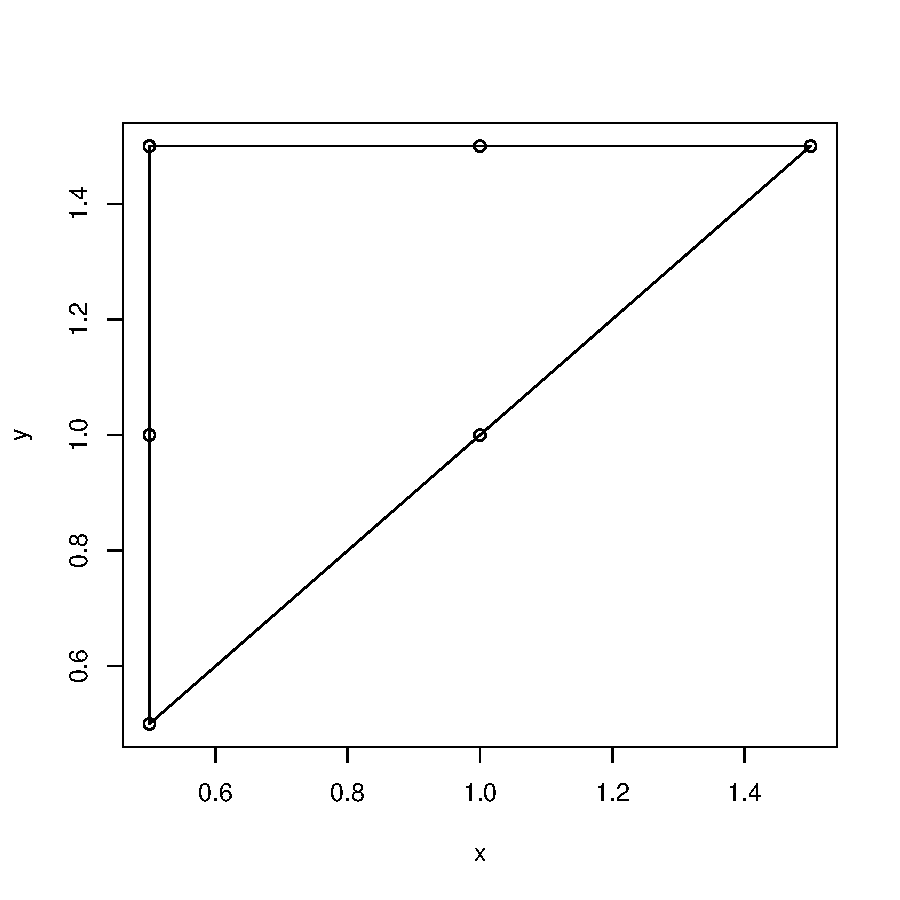
\includegraphics[width=3.5cm]{fig/it2.pdf} &
			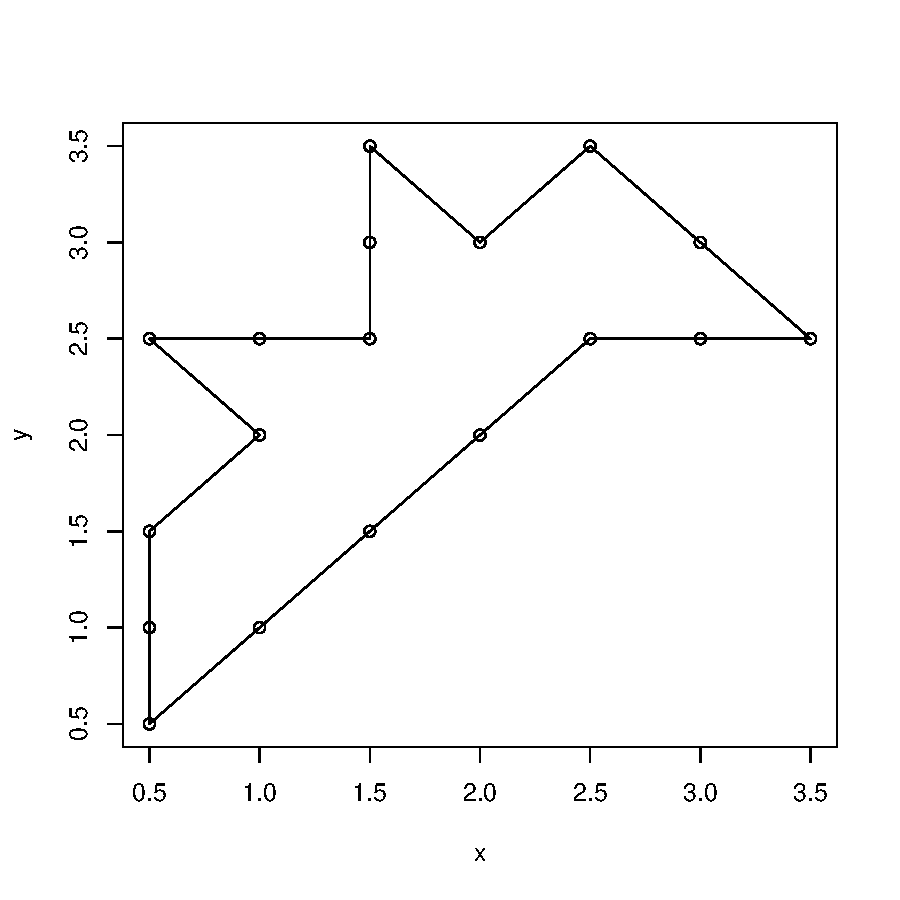
\includegraphics[width=3.5cm]{fig/it4.pdf} \NN
			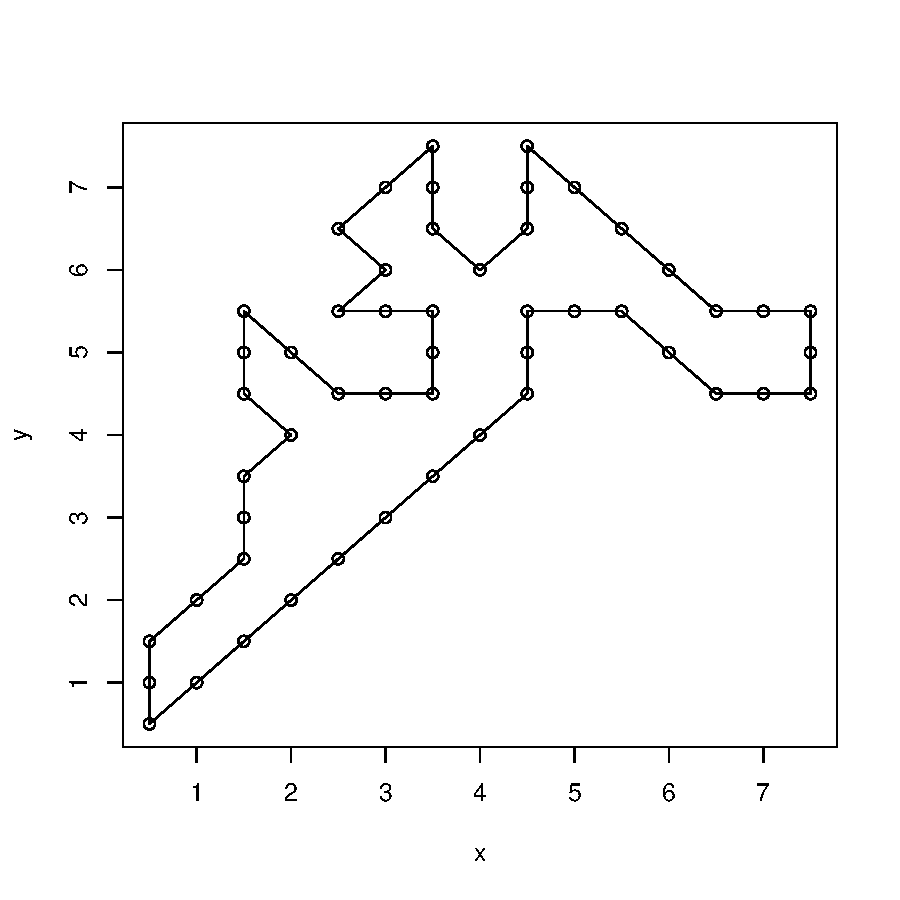
\includegraphics[width=3.5cm]{fig/it8.pdf} &
			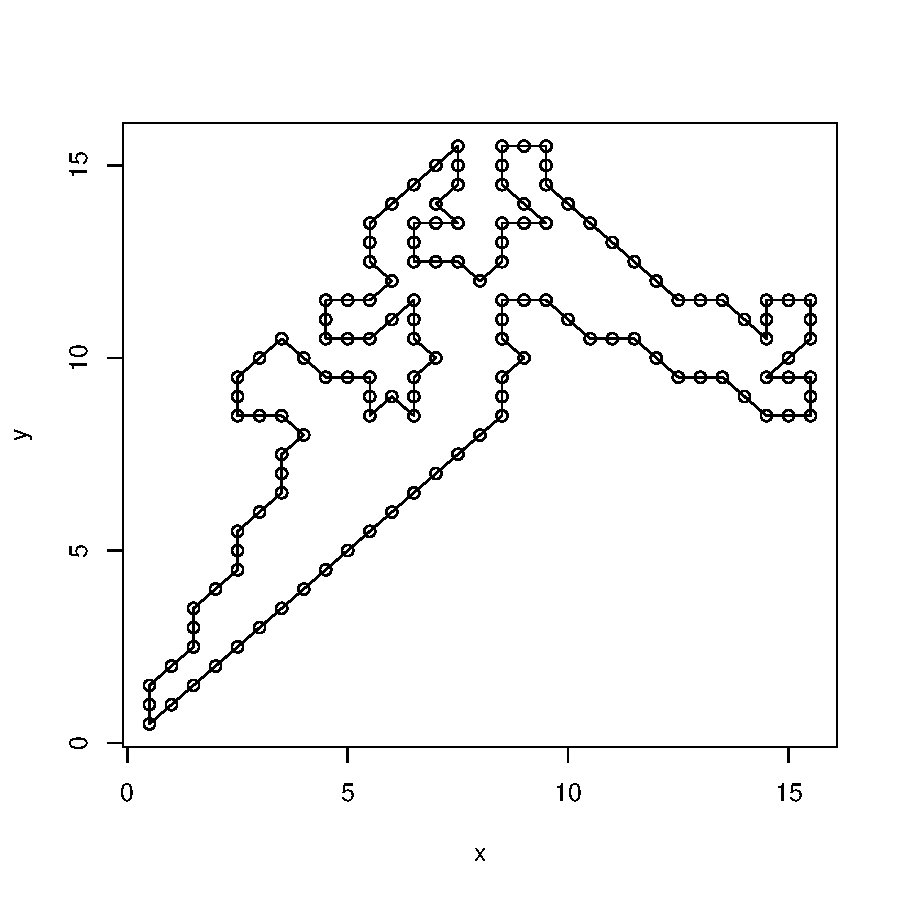
\includegraphics[width=3.5cm]{fig/it16.pdf} 
			\LL}


When the first iteration is finished we can use earlier blocks to calculate an approximation of the shortest tour at a smaller scale. We can divide all the blocks in four subblocks to study the problem at a smaller scale. Instead of iterating over all the subblocks in the image, which can be quite time consuming at a very small scale, only the blocks which are contains at least one city in the previous estimated shortest tour are used in the calculation. This limits the needed memory in the order of the size of the problem.

The information which is retrieved from the previous scale are the crossing points of the previous optimal path through the block. This optimal path can be seen in figure \ref{fig:renormalization}B.  These crossing points are at the places, where the edges of the path, pass the borders of one of the cells. This is illustrated in figure \ref{fig:renormalization}C. These crossing points, precalculated during the preprocessing stage, are used as start and ending point in the subblock. The optimal path between the starting and endpoint is retrieved, and placed in the subblock. The subblock is now a block on its own again, and can be used in the next scale.

\subsection{Retrieving the estimate of the shortest tour}
These process, which looks like zooming in on a microscope, is repeated until we reach unity. Unity is defined as the case where each cell has at most one city in it. Now we can directly retrieve our estimation of the shortest path. In figure \ref{fig:iterations} the first four iterations of the algorithm on $d198.tsp$ is shown. What is clear from this picture is that the route is refined in each iteration, until it exactly maps on the estimation  of the shortest optimal tour.

\subsection{Parallelization}
This algorithm can be extended for parallel execution. We did not perform this extension, but we have a suggestion of how to do this. The foundation for parallelism is in the observation that if we decrease to a smaller scale, we divide all the blocks into four subblocks independently. So if the code needs to be parallelized you take the following steps:

\begin{enumerate}
\item First perform some iterations on a single process. This is done until there are sufficient number of blocks for all the processes
\item Distribute the blocks over the processes, each process should have one connected part of the tour.
\item Each process can now recursively divide these blocks into subblocks, until unity is reached.
\item The cities which are visited in the part of a single process are retrieved and send back to the initiating process. These one can collect the data and output the total tour.
\end{enumerate}

This approach has a high potential of parallelism, since no communication is needed. Their is a pitfall however. If the blocks are shared equally it does not have to mean that the work is equally divided. In a worst case scenario a small group of processes can have a large set of all the cities. This problem can be reduced if there is a process which performs load balancing by shifting blocks, or sending one small set of blocks to a process at the time.
% vim:ft=tex:spell spelllang=en:autoindent
